\documentclass[a4paper,12pt]{article}
\usepackage{amssymb}
\usepackage{amsmath}
\usepackage[utf8]{inputenc} % Umlaute
\usepackage[ngerman]{babel} % Umlaute
\usepackage[T1]{fontenc}    % Umlaute
\usepackage[margin=2.5cm]{geometry}
\usepackage{booktabs}
\usepackage{lmodern}
\usepackage{titlesec}
\usepackage{longtable}
% Notwendig für Links im Text
\usepackage{hyperref}
%%\usepackage{svg}
% glossar, see http://en.wikibooks.org/wiki/LaTeX/Glossary
% muss NACH hyperref geladen werden, sonst funktionieren die Links nicht
\usepackage[toc]{glossaries}

% Kompatibilität
\ifx\pdftexversion\undefined
\usepackage[dvips]{graphicx}
\else
\usepackage[pdftex]{graphicx}
\DeclareGraphicsRule{*}{mps}{*}{}
\fi
\setlength{\parindent}{0pt}


%irgendwas mit section formatierung (titlesec package)
\titleformat{\paragraph}[hang]{\normalfont\normalsize\bfseries}{\theparagraph}{1em}{}
%%%%%%%%%%%%%%%%%%%%%%%%%%%%%%%%%%%%%%%%%%%%%%%%%%%%%%%%%%%%%%%%%%%%%%
% Variablen                                 						 %
%%%%%%%%%%%%%%%%%%%%%%%%%%%%%%%%%%%%%%%%%%%%%%%%%%%%%%%%%%%%%%%%%%%%%%
\newcommand{\authorName}{Tec O'Brain (Entwickler: David Höglinger, Jan Ettrich, Erwin Müller, Benedikt Rittner, Valentin Quapil)}
\newcommand{\auftraggeber}{Karlsruhe Institute of Technology (Teco)}
\newcommand{\auftragnehmer}{\authorName}
\newcommand{\projektName}{Implementierung Earables}
\newcommand{\tags}{\authorName, Architektur, Implementierung, KIT, Informatik, PSE}
\newcommand{\documentVersion}{1.0}
\title{\projektName}
\date{\today}
\author{Tec O'Brain}

%%%%%%%%%%%%%%%%%%%%%%%%%%%%%%%%%%%%%%%%%%%%%%%%%%%%%%%%%%%%%%%%%%%%%%
% PDF Meta information                                 				 %
%%%%%%%%%%%%%%%%%%%%%%%%%%%%%%%%%%%%%%%%%%%%%%%%%%%%%%%%%%%%%%%%%%%%%%
\hypersetup{
  pdfauthor   = {\authorName},
  pdfkeywords = {\tags},
  pdftitle    = {\projektName)}
}

%%%%%%%%%%%%%%%%%%%%%%%%%%%%%%%%%%%%%%%%%%%%%%%%%%%%%%%%%%%%%%%%%%%%%%
% Create a shorter version for tables. DO NOT CHANGE               	 %
%%%%%%%%%%%%%%%%%%%%%%%%%%%%%%%%%%%%%%%%%%%%%%%%%%%%%%%%%%%%%%%%%%%%%%
\newcommand\addrow[2]{#1 &#2\\ }

\newcommand\addheading[2]{#1 &#2\\ \hline}
\newcommand\tabularhead{\begin{tabular}{lp{13cm}}
\hline
}

\newcommand\addmulrow[2]{ \begin{minipage}[t][][t]{2.5cm}#1\end{minipage}%
   &\begin{minipage}[t][][t]{8cm}
    \begin{enumerate} #2   \end{enumerate}
    \end{minipage}\\ }

\newenvironment{usecase}{\tabularhead}
{\hline\end{tabular}}

\usepackage{microtype}
%%%%%%%%%%%%%%%%%%%%%%%%%%%%%%%%%%%%%%%%%%%%%%%%%%%%%%%%%%%%%%%%%%%%%%
% GLOSSARY ENTRIES                 	                              	 %
%%%%%%%%%%%%%%%%%%%%%%%%%%%%%%%%%%%%%%%%%%%%%%%%%%%%%%%%%%%%%%%%%%%%%%


%%%%%%%%%%%%%%%%%%%%%%%%%%%%%%%%%%%%%%%%%%%%%%%%%%%%%%%%%%%%%%%%%%%%%%
% THE DOCUMENT BEGINS             	                              	 %
%%%%%%%%%%%%%%%%%%%%%%%%%%%%%%%%%%%%%%%%%%%%%%%%%%%%%%%%%%%%%%%%%%%%%%
\begin{document}
\pagenumbering{roman}
\begin{titlepage}
\maketitle
\thispagestyle{empty} % no page number

\begin{verbatim}












\end{verbatim}


  \begin{tabular}[t]{p{4 cm}p{8 cm}}
	Projekt:       & \projektName \\[1.2ex]
	Auftraggeber:  & \auftraggeber\\[1.2ex]
	Auftragnehmer: & \auftragnehmer\\[1.2ex]
  \end{tabular}


\begin{tabular}[t]{|p{4 cm}|p{8 cm}|}
\hline
\textbf{Datum} & \textbf{Autor(en)} \\
\hline
\hline
\today & \authorName \\
\hline
\end{tabular}
\end{titlepage}
         % Deckblatt.tex laden und einfügen
\setcounter{page}{2}
\tableofcontents          % Inhaltsverzeichnis ausgeben
\clearpage
\pagenumbering{arabic}
%%%%%%%%%%%%%%%%%%%%%%%%%%%%%%%%%%%%%%% CONTENT %%%%%%%%%%%%%%%%%%%%%%%%%%%%%%%%%%%%%%%%%%%%%%%

\section{Einleitung}
%erwin:
%% massenfingersaugaktion
% gruppenzusammenarbeit, nuget, änderungen nur klein,
% in bennjis präsi nachschauen und mit zahlen flexen. frag benji dass er dir die Präsentation schickt


%%%%%%%%%%%%%%%%%%%%%% !!!!!!!!!!!!  struktur - Schema (runde Klammern = optional)
%
\section{Schema für Probleme und Änderungen am Entwurf}
\subsection{<<Bereich>>}
\subsubsection{<<Um was geht es>>}
\paragraph{Beschreibung}
<<Beschreibung>>
\paragraph{
  Änderung(en) (von ...) in Klasse(n) ... \\
  ODER \\
  Hinzugefügt in Klasse(n)... \\
  ODER \\
  Entfernen (von ...) in Klasse(n) ... (was nie vorkommt glaube ich) }
(<<kurze Erläuterung>>)
\begin{itemize}
  \item[+ ODER $-$] <<neues Attribut in UML-Notation>> (bei komplettem Austausch von z.B. Methode und Property: \textit{ersetzt} <<altes Attribut>>)
\end{itemize}
%
%%%%%%%%%%%%%%%%%%%%%%%%%% !!!!!!!!!!!!!!!
\section{Implemetierung der Erkennungsalgorithmen}
\section{Probleme und Änderungen am Entwurf}
\subsection{Bibliothek}

\subsubsection{Umgang mit Exceptions}
\paragraph{Beschreibung}
Es war geplant, dass die meisten Schnittstellen der Bibliothek ein Boolean zurückgeben, der true ist, falls die Anweisung korrekt durchgeführt werden konnte und false , falls es Komplikationen gab.\\
Um besser auf Fehler und Exceptions zu reagieren macht es mehr Sinn, dass diese Methoden nichts zurückgeben sind und im Fehlerfall Exceptions schmeißen.\\
Dies wurde umgesetzt, falls sich der Nutzer der Schnittstelle IEarablesConnection mehrmals verbinden will, keine Verbindung aufgebaut werden konnte, eine ungültige SampleRate angegeben wurde (Werte zwischen 1 und 100 sind erlaubt) oder eine Aktion ausgeführt werden soll, die bereits eine Verbindung voraussetzt, aber es existiert keine Verbindung.

\paragraph{Änderungen in Klasse IEarablesConnection}
Folgende Methoden haben nicht mehr den Rückgabetypen bool sondern void und schmeißen im Fehlerfall Exceptions:
\begin{itemize}
	\item[+] DisconnectFromDevice(): bool
	\item[+] StartSampling(): bool
	\item[+] StopSampling(): bool
\end{itemize} 
\paragraph{Hinzugefügte Exceptions}
Folgende Exception-Klassen mussten ergänzt werden:
\begin{itemize}
	\item[$-$] AllreadyConnectedException
	\item[$-$] ConnectionFailedException
	\item[$-$] InvalideSampleRateException
	\item[$-$] NoConnectionException
	\item[$-$] ChecksumException %man könnte noch überlegen die Rechtschreibfehler aus den AlreadyConnectedException und InvalidSampleRateException raus zu nehmen, müsste man dann aber auch konsequent im code so machen.
\end{itemize}
Die Exceptions werden geschmissen, falls bereits ein Gerät verbunden ist, keine Verbindung aufgebaut werden kann, der Wert der eingegebenen Samplerate nicht im richtigen Bereich (zwischen 1 und 100) liegt oder keine Verbindung vorhanden ist, diese aber benötigt würde (z.B. um das Sampling zu starten).

\subsubsection{Properties eingeführt}
\paragraph{Beschreibung}
\paragraph{Änderungen in Klasse IEarablesConnection}
In einigen Fällen gibt es nun keine Get/Set Methoden mehr. Sie wurden durch Properties ersetzt.
Folgende Properties sind als Attribute dazugekommen:
\begin{itemize}
	\item[+] Connected (\textit{ersetzt } die Methode IsConnected(): bool)
	\item[+] IsBluetoothActive  (\textit{ersetzt } die Methode IsBleutoothActive(): bool)
	\item[+] SampleRate  \textit{ersetzt } die Methode SetSamplingrate(heat: int): bool)
	\item[+] AccLPF  (\textit{ersetzt} SetLowPassFilterAccelerometer, GetLowPassFilterAccelerometer)
	\item[+] GyroLPF  (\textit{ersetzt} SetLowPassFilterGyroscope, GetLowPassFilterGyroscope)
	\item[+] BatteryVoltage  (\textit{ersetzt } die Methode GetBatteryVoltage(): float)
\end{itemize}

\paragraph{Hinzugefügt in Klasse EarablesConnection}
Zusätzlich zu den vererbten Änderungen ergeben sich folgende neue private Methoden:
\begin{itemize}
	\item[$-$] CheckIsBluetoothActive(): void
	\item[$-$] GetAccelerometerLPF(): LPF\_Accelerometer
	\item[$-$] SetAccelerometerLPF(LPF\_Accelerometer value): void
	\item[$-$] GetGyroscopeLPF(): LPF\_Gyroscope
	\item[$-$] SetGyroscopeLPF(LPF\_Gyroscope value): void
	\item[$-$] GetBatteryVoltageFromDevice(): void
	\item[$-$] initBatteryVoltage(): Task
\end{itemize}
  Hierbei wird GetBatteryVoltageFromDevice automatisch aufgerufen, wenn sich die BatteryVoltage der Earables ändert und überträgt den aktuellen Wert in das BatteryVoltage Attribut.\\
  Die Methode initBatteryVoltage liest den BatteryVoltage Wert der Earables zum ersten Mal aus, falls sie abgefragt werden sollte, bevor sie sich das erste Mal aktualisiert hat.

\subsubsection{Kapselung von Attributen der Bibliothek}
\paragraph{Beschreibung}
Für die Attribute config und characteristics ist es in Betracht der Datenkapselung sinnvoller, sie private zu halten. Sie werden von außen nicht direkt benötigt.
\paragraph{Änderungen der Sichtbarkeit in Klasse IEarablesConnection}
\begin{itemize}
	\item[$-$] config
	\item[$-$] characters
\end{itemize}


\subsubsection{Namensänderungen bei Enums}
\paragraph{Beschreibung}
Die Enums können nicht mit Zahlen beginnen. Daher mussten sie umbenannt werden.
\paragraph{Änderungen in den Enums LPF\_Accelerometer und LPF\_Gyroscope}
Die Werte der Enums beginnen nun nicht mehr mit der Zahl sondern mit Hz. \\
Beispielsweise wird statt 10Hz jetzt Hz10 verwendet.

\subsubsection{Übergabe der Geräte beim Scanvorgang}
\paragraph{Beschreibung}
Es war ursprünglich gedacht, dass die StartScanning Methode eine Liste mit alle gefundenen Devices zurück gibt. Die Liste, die zurückgegeben wurde war aber immer leer, da Methoden aus dem Plugin BLE benutzt wurden, die asynchron laufen. So wurde zuerst die Liste zurückgegeben und danach wurde sie befüllt. Nach etlichen gescheiterten Versuchen auf die Threads und Tasks zu warten haben wir uns dafür entschieden jedes Mal ein Event zu schmeißen, wenn ein neues Device gescannt wurde. Die Argumente des Events beinhalten das neue Device.
\paragraph{Hinzugefügt in der Klasse IEarablesConnection}
\begin{itemize}
	\item[+] event NewDeviceFound: EventHandler<NewDeviceFoundArgs> 
\end{itemize}
\paragraph{Klasse NewDeviceFound hinzugefügt}
\begin{itemize}
	\item[+] Device: IDevice
	\item[+] <<create>> NewDeviceFound(device :IDevice)
\end{itemize}

\subsubsection{Static Methoden in der Klasse IEarablesConnection}
\paragraph{Beschreibung}
Es wurde angenommen, dass die Methoden, die auf die Events der Earables reagieren static sein müssen. Diese Annahme war falsch.
\paragraph{Änderungen in der Klasse IEarablesConnection}
Die folgenden Methoden sind nun nicht mehr statisch:
\begin{itemize}
  \item[+]OnValueUpdatedIMU():void
  \item[+]OnPushButtonPressed():void
  \item[+]OnDeviceConnected():void 
\end{itemize}


\subsubsection{Reaktion auf Verbinden und Trennen von Devices}
\paragraph{Beschreibung}
Es wurden zwei Methoden hinzugefügt, um den Connectionstate des Smartphones mit Hilfe des DeviceConnectionStateChanged Events weiterzuleiten.\\
 Sie werden aktiviert, wenn sich die Earables mutwillig vom Device trennen oder die Verbindung unterbrochen wird.
\paragraph{Hinzugefügt in der Klasse EarablesConnection}

\begin{itemize}
	\item[-] OnDeviceDisconnected(object sender, DeviceEventArgs args): void 
	\item[-] OnDeviceConnectionLost(object sender, DeviceErrorEventArgs args): void
\end{itemize}

\subsubsection{Funktionsweise der Klasse IMUDataExtractor}
\paragraph{Beschreibung}
Hier waren aus verschiedenen Gründen Änderungen nötig: 
Die Methode ExtractIMUDataString benötigt für die Berechnung der Sensordaten zusätzlich noch den Offset. Dieser wird nun als vierter Parameter übergeben.\\
 Die Skalierungsfaktoren, die als Parameter übergeben werden können nicht nur ganzzahlig sein, hier sind Fließkommazahlen sinnvoller.\\
Die Klasse wurde der Vollständigkeit halber um zwei Methoden ergänzt, die die Range des Accelerometers und des Gyroscopes aus dem entsprechenden Bytearray ermitteln.
\paragraph{Änderungen in der Klasse IMUDataExtractor}
\begin{itemize}
  \item[+] \underline{ExtractIMUDataString(byteString: int, accScaleFactor: double,} \\
  \underline{GyroScaleFactor: int, byteOffset: byte[])} 
	\item[+] \underline{ExtractIMUScaleFactorAccelerometer(byteString: int): double}
	\item[+] \underline{ExtractIMUScaleFactorGyoscope(byteString: int): int}
\end{itemize}
\paragraph{Hinzugefügt in der Klasse IMUDataExtractor}
\begin{itemize}
  \item[+] \underline{ExtractIMURangeAccelerometer(byte[] bytes): int} 
	\item[+] \underline{ExtractIMURangeGyroscope(byte[] bytes): double} 
\end{itemize}
\subsubsection{Charakteristik umbenannt}
\paragraph{Beschreibung}
Eine Charakteristik wurde umbenannt.
\paragraph{Änderungen in der Klasse Constants}
\begin{itemize}
	\item[-] OFFSET\_CHAR (\textit{ersetzt}  IMU\_FULL\_SCALE\_RANG\_CHAR) %uml?
\end{itemize}
\paragraph{Änderungen in der Klasse Characteristics}
\begin{itemize}
	\item[-] OffsetChar (\textit{ersetzt} IMUScaleRangeChar) %uml?
\end{itemize}

\subsubsection{Verbindungsüberprüfung}
\paragraph{Beschreibung}
Um festzustellen ob eine Verbindung zu einem Device besteht wurde eine Methode hinzugefügt
\paragraph{Ergänzungen in der Klasse EarablesConnection}
\begin{itemize}
	\item[-]  CheckConnection():void  
\end{itemize}
Sie wird am Anfang aller  Methode, die eine Verbindung voraussetzen, aufgerufen und prüft ob eine Verbindung existiert. Falls keine existiert schmeißt sie eine die Exception NoConnectionException.

\subsubsection{Zwischenpeichern der Scalierungsfaktoren von Acc und Gyro}
\paragraph{Beschreibung}
Um das Bytearray des IMU auszuwerten benötigt man die Scalefactoren für den Accelerometer und für das Gyroscope. Wenn man diesen aber erst in der Methode OnValueUpdatedIMU ausliest stürzt die App ab, da die Methode jedes mal aufgerufen wird, wenn neue IMUDaten anliegen, was bis zu 100 mal pro Sekunde passieren kann. Das liegt daran, dass das Auslesen der Charakteristiken mit Hilfe von asynchronen Methoden aus dem Plugin.BLE geschieht. Deswegen werden die Scalefactoren bereits beim Starten des Samplings ausgelesen und müssen irgendwo zwischengespeichert werden. Dafür wurden in der Klasse ConfigContainer zwei Attribute AccScaleFactor und GyroScaleFactor hinzugefügt. Außerdem enthält sie zusätzlich noch eine Methode um zu überprüfen, ob die Samplingrate im gültigen Wertebereich liegt. Das gleiche Problem ergab sich auch beim lesen des Offset Bytearrasy. Dieser wird jetzt in einer privaten Variable in der Klasse EarablesConnection gespeichert, da es sich hierbei nicht um eine Konfiguration handelt.

\paragraph{Ergänzungen in der Klasse EarablesConnection}
\begin{itemize}
	\item[$-$] byteOffset: byte[]
\end{itemize}

\paragraph{Ergänzungen in der Klasse ConfigContainer}
\begin{itemize}
	\item[+] AccScaleFactor: int 
	\item[+] GyroScaleFactor: int
	\item[$-$]  setSamplingRate(int rate): void 
\end{itemize}
Beim setzten des Samplingrate Propertys wird die Methode setSamplingRate ausgeführt und stellt sicher, dass nur gültige Werte angenommen werden.

\subsubsection{Testmethoden hinzugefügt}
\paragraph{Beschreibung}
Die Scalefactoren hängen von der gewählten Range des Accelerometers und des Gyroscopes ab. Um zu testen ob der richtige Wert in die  Earables geschrieben wird gibt es nun zusätzlich zwei Methoden, die die Range setzen und weitere zwei um die Range von den Earables zu lesen.
Außerdem wird beim setzen der LPF, in den configs gespeichert auf welchen Wert sie momentan gesetzt sind. Beim Auslesen wird also nicht der Wert von den Earables gelesen sonder der Wert der in den configs steht. Das hat den selben Grund weshalb wir die gefundenen Devices, beim scannen, nicht als Liste zurückgeben. Um den aktuellen LPF der Earables auszulesen benutzen wir wieder asynchrone Methoden aus dem Plugin.BLE. Das heißt der Wert des LPF wird erst zurückgegeben und dann erst ausgelesen, was das Ergebnis verfälscht. Um das zu vermeiden werden die Werte für die LPF nicht aus den Earables ausgelesen sondern aus den Configs, in denen sie gespeichert wurden. Für Testzwecke wurden jedoch trotzdem zwei Methoden implementiert, die die Werte für die LPF direkt aus den Earables lesen. Diese Methoden werden auch in der BibTestApp zum auslesen verwendet.

\paragraph{Ergänzungen in der Klasse EarablesConnection}
\begin{itemize}
	\item[$-$] setAccelerometerRange(range :int): void
	\item[$-$] setGyroscopeRange(range: int): void
	\item[$-$ ] getAccelerometerLPFFromDevice(): void
	\item[$-$ ] getGyroscopeLPFFromDevice(): void
\end{itemize}
Ermöglichen es die Range zu setzen und den LPF aus den Earables auszulesen. Die Methoden um die Range auszulesen befinden sich in der Klasse IMUDataextractor. Die Methoden zum auslesen des  LPF schreiben den LPF in eine Variable. Bei Verwendung dieser Methoden müssen die Variablen vorher global deklariert werden, um auf sie zuzugreifen zu können. Da wir die Methoden nicht benutzen und sie nur zum testen da sind existieren diese globalen Variablen in unsere Bibliothek nicht.

\subsubsection{Checksummen Überprüfung}
\paragraph{Beschreibung}
Die Bytearrays beinhalten ein Byte, in dem eine Checksumme gespeichert wird. Sie setzt sich aus der Addition der Restlichen Bytes zusammen. 

\paragraph{Ergänzungen in der Klasse EarablesConnection}
\begin{itemize}
	\item[$-$] CheckChecksum(bytes: byte[]): void
	\item[$-$] CheckIMUChecksum(bytes: byte[]): void
\end{itemize}
Beim erhalten des Bytearrays überprüfen wir nun ob diese mit dem Sollwert übereinstimmt oder ob bei der Übertragung ein paar Bits verloren gegangen sind. Falls es keine Übereinstimmung gibt wird eine Exception geschmissen. Es gibt eine Methode die sich für die Überprüfung aller Bytearrays eignet außer für die Überprüfung des IMUData Bytearrays da es leicht anders aufgebaut ist als die restlichen Bytearrays.

% durchlesen bis hier valle
\subsection{Erweiterungsmodul}

\subsection{Model (andere Bestandteile)}

\subsubsection{Datenbank Service}
\paragraph{Beschreibung}
Ursprünglich war es geplant die Datenbank asynchrons zu implementieren. Dies ist nicht nötig für unsere Anwendung, weswegen wir auf eine synchrone Datenbank gewechselt sind. Das ergibt einen klaren Kontrollfluss, welcher besser nachvollziehbar ist. Die Synchronisierung schadet nicht der Performance, da keine großen Datenbankzugegriffe getätigt wern wird, um Endlosschleifen beim Aktualisieren der Attribute zu verhindern.

\paragraph{Änderungen in den Klassen IDataBaseConnection und DataBaseConnection}
\begin{itemize}
	\item[+] GetAllEntriesAsync(): Namen in GetAllEntries() \textit{geändert} und Rückgabewert in List<DBEntry> \textit{geändert}.
	\item[+] GetMostRecentEntriesAsync(): Namen in GetMostRecentEntries() \textit{geändert} und Rückgabewert in List<DBEntry> \textit{geändert}.
\end{itemize}
\paragraph{Attributänderung der Klassen DataBaseConnection}
\begin{itemize}
	\item[$-$] \_database : SQLiteConnection als synchrone Datenbank \textit{hinzugefügt}.
\end{itemize}

\paragraph{Beschreibung}
Zum Speichern der DBEntries wurde eine neue Klasse namens DBEntryToSave hinzugefügt, da die Datenbank keine komplexeren Datentypen speichern kann, sondern nur primitive. DBEntryToSave ist abgekapselt im Datenbank Service. 

\paragraph{Hinzufügen der Klasse DBEntryToSave}
\begin{itemize}
	\item[+] DateTime: DateTime: Attribut \textit{hinzugefügt}. Dient als Primary key, welcher in der Datenbank gespeichert wird.
	\item[+] TrainingsDataAsString: string: Attribut \textit{hinzugefügt}. Speichert die Trainingsdaten als string, welcher in der Datenbank gespeichert wird. Dieser bildet sich aus dem Dictionary TrainingsData der Klasse DEntry.
\end{itemize}

\paragraph{Änderungen in Klasse DBEntry}

\begin{itemize}
	\item[+] const StepAmountIdentifier: string: Identifier für das Dictionary für die Schrittanzahl
	\item[+] const PushAmountIdentifier: string: Identifier für das Dictionary für die Liegestützenanzahl
	\item[+] const SitUpAmountIdentifier: string: Identifier für das Dictionary für die SitUpanzahl
	\item[+] ConvertToDBEntryToSav()e: DBEntryToSave: Methode \textit{hinzugefügt} um die Instanz in eine Instanz vom Type DBEntryToSave. 
	\item[+] ParseDbEntry(): Nun überladen mit den Parametern vom Typ DBEntryToSave und vom Typ string.
	
\end{itemize}

\subsection{Views und ViewModel}

\subsubsection{Commandstruktur bei Modi}
\paragraph{Beschreibung}
Beim Starten eines Modus durch Drücken des Start Buttons wurde ursprünglich ein Command direkt das ViewModel gesendet und dort die StartActivity Methode aufgerufen. Da aber beim Starten auch die View gewechselt werden soll und dies aus dem ViewModel nicht umsetzbar ist, muss das Drücken des Start Buttons zunächst im Codebehind der zugehörigen View behandelt und dann weiter an das ViewModel delegiert werden. 
\paragraph{Änderungen in Klasse BaseModeViewModel}
\begin{itemize}
	\item[+] StartActivityCommand: ICommand und StopActivityCommand: ICommand \textit{entfernt}.
	\item[+] \textit{abstract} StartActivity(): bool und \textit{abstract} StopActivity(): bool Sichtbarkeit von protected auf public \textit{verändert} und Rückgabewerte auf bool \textit{geändert}.
	\item[\#] CheckConnection(): bool Rückgabetyp zu bool \textit{geändert}.
\end{itemize}
\paragraph{Änderungen in Klassen CountViewModel, StepViewModel und ListAndPerformViewModel}
Bei den Kindklassen verändern sich analog die vererbten StartActivity und StopActivity Methoden.
\begin{itemize}
	\item[+] StartActivity(): bool und StopActivity(): bool Sichtbarkeit von protected auf public \textit{verändert} und Rückgabewerte auf bool \textit{geändert}.
	\item[+] UpdateFrequency(): void Sichtbarkeit von private auf public geändert (\textbf{Nur StepModeViewModel}). 
\end{itemize}
\paragraph{Änderungen in CountModePage, StepModePage und ListenAndPerformPage}
\begin{itemize}
	\item[-] ViewModel: (jeweiliger Type)ViewModel \textit{hinzugefügt}.
	\item[+] OnStartButtonClicked (sender: object, args: EventArgs): void \textit{hinzugefügt}.
	\item[+] ChangeView (): void \textit{hinzugefügt}.
\end{itemize}
\paragraph{Änderungen in CountModeActivePage, StepModeActivePage und ListenAndPerformActivePage}
\begin{itemize}
	\item[-] ViewModel: (jeweiliger Type)ViewModel \textit{hinzugefügt}.
	\item[+] OnStopButtonClicked (sender: object, args: EventArgs): void \textit{hinzugefügt}.
	\item[+] ChangeView (): void \textit{hinzugefügt}.
\end{itemize}

\subsubsection{Wrapperklasse für Activities}
\paragraph{Beschreibung}
Um die Anzahl lokaler Attribute und Fallunterscheidungen zu verringern, wurde eine Wrapperklasse für Activities  erstellt. Damit kann dynamisch auf den Namen der Activity sowie deren Counter und der vom Servicemanager gelieferten Analyse zugegriffen werden. Sie implementiert außerdem die Schnittstelle INotifyPropertyChanged, da einige Attribute der Klasse per Databinding angezeigt und während eines laufendes Modus verändert werden.
\paragraph{Hinzufügen der Klasse ActivityWrapper}
\begin{itemize}
	\item[+] \_activity: Activity \textit{hinzugefügt}.
	\item[+] Name: string \textit{hinzugefügt}.
	\item[+] Amount: int \textit{hinzugefügt}.
	\item[-] \_counter: int \textit{hinzugefügt}.
	\item[-] Counter: int \textit{hinzugefügt}.
	\item[+] <<create>> ActivityWrapper(name: string, activity: Activity, amount: int) \textit{hinzugefügt}.
	\item[+] <<create>> ActivityWrapper(name: string, activity: Activity) \textit{hinzugefügt}.
	\item[\#] OnPropertyChanged([CallerMemberName]): void \textit{hinzugefügt}.
\end{itemize}
\paragraph{Änderungen in CountModeViewModel}
\begin{itemize}
	\item[+] \_pushUpActivityWrapper: ActivityWrapper \textit{hinzugefügt}.
	\item[+] \_sitUpActivityWrapper: ActivityWrapper \textit{hinzugefügt}.
	\item[+] \_comingSoon: ActivityWrapper \textit{hinzugefügt}.
	\item[+] PossibleActivities: ObservableCollection<ActivityWrapper> Datentyp der Listenelemente von string zu ActivityWrapper\textit{geändert}.
	\item[+] SelectedActivity: ActivityWrapper Datentyp von string zu ActivityWrapper \textit{geändert}.
\end{itemize}
\paragraph{Änderungen in ListenAndPerformViewModel}
\begin{itemize}
	\item[+] ActivityList: ObservableCollection<ActivityWrapper> Datentyp der Listenelemente von string zu ActivityWrapper\textit{geändert}.
	\item[+] SelectedActivity: ActivityWrapper Datentyp von string zu ActivityWrapper \textit{geändert}.
	\item[+] ActiveActivity: ActivityWrapper \textit{hinzugefügt}.
	\item[-] \_activeActivity: ActivityWrapper \textit{hinzugefügt}.
 	\item[+] ActivityAmounts: OberservableCollection<int> \textit{entfernt}. 
\end{itemize}

\subsubsection{Data Binding Endlosschleife}
\paragraph{Beschreibung}
Im Entwurf wurde nicht berücksichtigt, dass jedes Attribut, welches per Data Binding an Viewelemente gebunden und nicht per default Two-Way binded ist,  auch ein äquivalentes privates Attribut benötigt wird, auf das bei den settern und gettern zugegriffen wird, um Endlosschleifen beim Aktualisieren der Attribute zu verhindern. 
\paragraph{Änderungen im StepModeViewModel}
\begin{itemize}
	\item[-] \_stepsDoneLastTime: int \textit{hinzugefügt} und Datentyp des public Attributs von string zu int geändert.
	\item[-] \_distanceWalkedLastTime: int \textit{hinzugefügt} und Datentyp des public Attributs von string zu int geändert.
	\item[-] \_lastDataTime: string \textit{hinzugefügt}.
	\item[-] \_stepCounter: int \textit{hinzugefügt}.
	\item[-] \_distanceWalked: int \textit{hinzugefügt}.
	\item[-] \_isRunning: bool \textit{hinzugefügt}.
	\item[-] \_stepFrequency: double \textit{hinzugefügt} und Datentyp des public Attributs von string zu double geändert.
\end{itemize}
\paragraph{Änderungen im CountModeViewModel}
\begin{itemize}
	\item[-] \_minutes: string \textit{hinzugefügt}. 
	\item[-] \_seconds: string \textit{hinzugefügt}.
	\item[-] \_milliseconds: string \textit{hinzugefügt}.
\end{itemize}
\paragraph{Änderungen im ListenAndPerformViewModel}
\begin{itemize}
	\item[-] \_minutes: string \textit{hinzugefügt}.
	\item[-] \_seconds: string \textit{hinzugefügt}.
	\item[-] \_milliseconds: string \textit{hinzugefügt}.
\end{itemize}

\subsubsection{Speichern der gesammelten Daten der Modi}
\paragraph{Beschreibung}
Das Speichern der ausgeführten Sit-ups, Push-ups oder gelaufenen Schritten wurde in eine neue Methode ausgelagert, um Fallunterscheidungen zu vermeiden.
\paragraph{Änderungen in Klassen CountViewModel, StepViewModel und ListAndPerformViewModel} 
\begin{itemize}
	\item[-] saveData(): void \textit{hinzugefügt}.
\end{itemize}

\subsubsection{Zwischenspeichern von Services}
\paragraph{Beschreibung}
Um die Übersichtlichkeit in Methoden zu wahren, werden häufig benutzte Services im Konstruktor einmalig vom Service Manager geholt und in einem Attribut gespeichert.
\paragraph{Änderungen in Klassen CountModeViewModel, StepModeViewModel und ListAndPerformViewModel} 
\begin{itemize}
	\item[-] \_activityManager: IActivityManager \textit{hinzugefügt}.
	\item[-] \_dataBaseConnection: IDataBaseConnection \textit{hinzugefügt} .
\end{itemize}

\subsubsection{Neue Event Methode für RunningEvents}
\paragraph{Beschreibung}
Der StepMode muss gleichzeitig von zwei Aktivitätsanalysen Events bekommen, von der RunningActivity und von der StepActivity. Wenn die OnActivityDone Methode bei beiden Event Handlern der Aktivitäten registriert wird, müssten mehrere Fallunterscheidungen und eine Auswertung der nicht implementierten ActivityArgs erfolgen. Stattdessen wird eine neue Methode hinzugefügt, sodass bei jedem Event Handler nur eine seperate Methode registiert ist.
\paragraph{Änderung im StepModeViewModel}
\begin{itemize}
	\item[+]  OnRunningDone(sender: object, args: ActivityArgs): void \textit{hinzugefügt}.
\end{itemize}

\subsubsection{Auslagerung der Registrierung im CountModeViewModel}
\paragraph{Beschreibung}
Um sicher zu gehen, dass der Nutzer beim Starten des Zählmodus eine gültige Aktivität ausgewählt hat, wird eine neue Methode hinzugefügt, die im Erfolgsfall auch die Event Methode des ViewModels beim korrekten Event Handler registriert.
\paragraph{Änderung im CountModeViewModel}
\begin{itemize}
	\item[-]  RegisterActivity(): bool \textit{hinzugefügt}.
\end{itemize}

\subsubsection{Progressbar im ListenAndPerformViewModel}
\paragraph{Beschreibung}
Zu besseren Visualisierung des Fortschritts des Nutzers während einer Trainingseinheit wurde eine Progressbar hinzugefügt. Diese wird mit einer Hilfsvariable nach der Ausführung einer Wiederholung einer Aktivität aktualisiert und resettet sich nach jedem abgearbeiteten Listeneintrag.
\paragraph{Änderungen im ListenAndPerformViewModel }
\begin{itemize}
	\item[-] Repetitions: int \textit{hinzugefügt}.
	\item[-] \_progress: double \textit{hinzugefügt}
	\item[+] ProgressLive: double \textit{hinzugefügt}
\end{itemize}
\paragraph{Änderung in ListenAndPerformActivePage}
\begin{itemize}
	\item[+] Progress: ProgressBar \textit{hinzugefügt}.
\end{itemize}

\subsubsection{Ablauf in ListenAndPerform}
\paragraph{Beschreibung}
Die Abarbeitung der vom Nutzer zusammengestellten Aktivitätsliste erfolgt nun vollständig auf Event Basis, anstelle innerhalb der DoActivity Methode. Die OnActivityDone Methode zählt nun nicht mehr nur immer einen Counter hoch, sondern prüft gleichzeitig auch, ob die festgelegte Anzahl an Wiederholungen gemacht wurde, um in dem Fall über den Iterator die nächste Aktivität aus der Liste zu holen. Die Zwischenspeicherung der bisher geleisteten Push-ups und Sit-ups regelt die neue Methode IncreaseResultCounter, welche von OnActivityDone aufgerufen wird. Die Methode CheckNextActivity ersetzt die DoActivity Methode und kümmert sich um das Registrieren der OnActivityDone Methode beim korrekten Event Handler. 
\paragraph{Änderungen im ListenAndPerformViewModel}
\begin{itemize}
	\item[-] CheckNextActivity(): void \textit{hinzugefügt}.
	\item[-] IncreaseResultCounter(): void \textit{hinzugefügt}.
	\item[-] DoActivity(): void \textit{entfernt}.
\end{itemize}
	
\subsubsection{Pause in ListenAndPerform}
\paragraph{Beschreibung}
Um den Ablauf einer Pause reibungslos zu ermöglichen wurde ein zusätzlicher Timer eingebaut, der nur aktiviert wird wenn der nächste Listeneintrag in der Aktivitätsliste eine Pause ist. Dabei wird in der CheckNextActivity Methode jede Sekunde ein Event an die neu hinzugefügte Methode OnTimedEvent gesendet. Diese Methode funktioniert dann analog zur OnActivityDone Methode und ruft die nächste Aktivität aus der Liste auf, wenn die Pausenzeit abgelaufen ist.
\paragraph{Änderungen im ListenAndPerformViewModel}
\begin{itemize}
	\item[-] PauseTimer: Timer \textit{hinzugefügt}.
	\item[-] OnTimedEvent(): void \textit{hinzugefügt}.
\end{itemize}

\subsubsection{Weitere Anzeigeelemente in Viewklassen}
\paragraph{Beschreibung}
Ergänzung einiger zusätzlicher Anzeigeelemente.
\paragraph{Änderungen in StepModePage}
\begin{itemize}
	\item[+] StepModeTrainingsDateLabel: Label \textit{hinzugefügt}.
	\item[+] StepModeLastStepsLabel: Label \textit{hinzugefügt}.
	\item[+] StepModeLastDistanceLabel: Label \textit{hinzugefügt}.
\end{itemize}
\paragraph{Änderungen in StepModeActivePage}
\begin{itemize}
	\item[+] StepModeStartDataTime: Label \textit{hinzugefügt}.
	\item[+] CurrentDate: Label \textit{hinzugefügt}.
	\item[+] StepModeUnbindedStatusLabel: Label \textit{hinzugefügt}.
	\item[+] StepModeUnbindedStepsDoneLabel: Label \textit{hinzugefügt}.
	\item[+] StepModeUnbindedFrequencyLabel: Label \textit{hinzugefügt}.
	\item[+] DistanceWalkedLabel: Label \textit{entfernt}.
\end{itemize}
\paragraph{Änderungen in CountModePage}
\begin{itemize}
	\item[+] PossibleActivitiesLabel:Label \textit{hinzugefügt}.
\end{itemize}
\paragraph{Änderungen in ListenAndPerformActivePage}
\begin{itemize}
	\item[+] CurrentActivityUnbindedLabel:Label \textit{hinzugefügt}.
\end{itemize}

\subsubsection{Überladung im ExceptionHandlingViewModel}
\paragraph{Beschreibung}
Das ExceptionHandlingViewModel ist ein statisches Singleton mit der zentralen Methode HandleException(error: Exception). Da wir nicht immer die Fehlermeldung der Exception werfen wollen haben wir uns dazu entschieden eine Standardfehlermeldung zu implementieren. Dazu haben wir die Methode HandleException überladen. Sie existiert jetzt auch ohne ein Argument, was der Standardfehlermeldung entspricht.
\paragraph{Änderung in ExceptionHandlinViewModel}
\begin{itemize}
	\item[+] HandleException(): void: Methodenüberladung hinzugefügt. Wirft eine Standardfehlermeldung in Form eines Displayalerts.
\end{itemize}

\subsubsection{Aktualisierung DataOverViewPage}
\paragraph{Beschreibung}
Bei der Standardimplementierung des Hamburgermenus wird bei der Navigation zu einer Seite nu beim ersten Aufruf eine Instanz erstellt. Die DataOverViewPage muss bei jedem Aufruf der Seite neu aktualisiert werden. Die Datenbankeinträge erhält sie von der Datenbank per Methodenaufruf. Um bei jedem Erscheinen neu zu aktualisieren, wurde sich bei dem EventHandler Appearing mit der neuen Methode OnAppearing registriert.

\paragraph{Änderung in DataOverViewModel}
\begin{itemize}
	\item[+] OnAppearing(sender: object, e: EventArgs): Eventmethode hinzugefügt, welche die Daten neu lädt.
\end{itemize}


\subsubsection{Verarbeitung des Import/Export}
\paragraph{Beschreibung}
Im Entwurf haben wir uns dazu entschieden,dass das ImportExportViewModel die komplette Verarbeitung des Importieren und Exportieren der Daten macht. Um eine Datei auszuwählen haben wir uns dazu entschieden einen CrossFilePicker zu benutzen. Dieser lässt den User auswählen, von wo/wohin geladen/gespeichert werden soll. Diese Funktionalität haben wir in das Codebehind von der page ImportExportPage verlegt.

\paragraph{Änderung in ImportExportViewModel}
\begin{itemize}
	\item[+] ExportData(path: FileData): Methode ExportData bekommt nun ein pfad in den es die zu exportierende Datei speichern soll.
	\item[+] ImportData(path: FileData): Methode ImportData bekommt nun ein pfad welcher angibt, wo die zu lesende Datei im Speicher liegt.
\end{itemize}

\paragraph{Änderung in ImportExportPage}
\begin{itemize}
	\item[$-$] ImportButton\_Clicked(): Eventmethode fürs reagieren auf den ImportButtonclick \textit{hinzugefügt}
	\item[$-$] ExportButton\_Clicked(): Eventmethode fürs reagieren auf den ExportButtonclick \textit{hinzugefügt}
	
\end{itemize}

\subsubsection{Aktualisierung ScanningDevices}
\paragraph{Beschreibung}
Das ScanningPopUp zeigt nach dem betätigen des Buttons 'Scan Devices' die Liste der gefundenen Geräte an. Sobald ein geeignetes Gerät gefunden wurde, soll die View geupdated werden (der Button 'Verbinden' wird enabled). Diese Logic beinhaltet das Codebehind der Seite PopUpScanningPage.

\paragraph{Änderung in PopUpScanningPage}
\begin{itemize}
	\item[+] UpdateList(sender: object, e: PropertyChangedEventArgs): Methode \textit{hinzugefügt}. Es handelt sich um eine Eventmethode, welche bei dem Update der DeviceList aufgerufe wird. Dise überprüft, ob die Liste leer ist und ändert dem entsprechend die View ab.
	\item[$-$] ConnectButton\_Clicked() : Methode \textit{hinzugefügt}. Dies ist eine Eventmethode, welche beim Betätigen des Connect button aufgerufen wird.
\end{itemize} 

\section{Implementierungsplan}
%benni
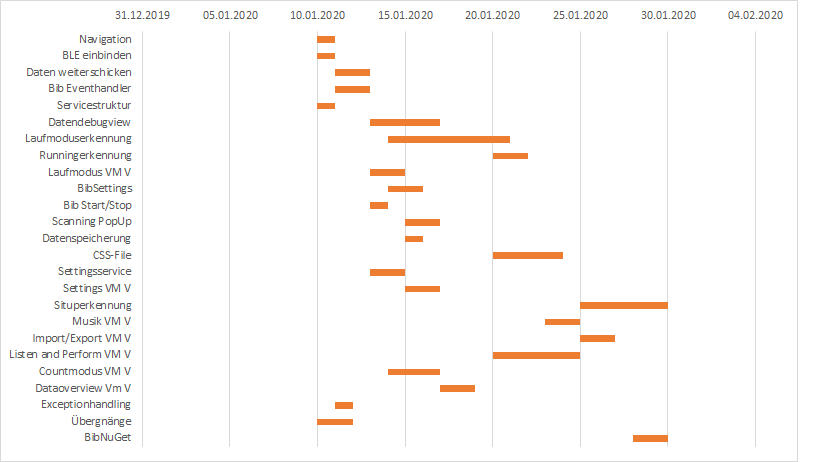
\includegraphics[width=\textwidth]{bilder/Implementierungsplan.png}
\section{Anhang}
die ganzen Verweise zum repo, nuget
%valle
%%%%%%%%%%%%%%%%%%%%%%%%%%%%%%%%%%%%%%% END CONTENT %%%%%%%%%%%%%%%%%%%%%%%%%%%%%%%%%%%%%%%%%%%


\printglossaries
\stepcounter{section}


\end{document}